%%%%%%%%%%%%%%%%%%%%%%%%%%%%%%%%%%%%%%%%%
% "ModernCV" CV and Cover Letter
% LaTeX Template
% Version 1.11 (19/6/14)
%
% This template has been downloaded from:
% http://www.LaTeXTemplates.com
%
% Original author:
% Xavier Danaux (xdanaux@gmail.com)
% Modified by:
% Antonius Torode
%
% License:
% CC BY-NC-SA 3.0 (http://creativecommons.org/licenses/by-nc-sa/3.0/)
%
% Important note:
% This template requires the moderncv.cls and .sty files to be in the same 
% directory as this .tex file. These files provide the resume style and themes 
% used for structuring the document.
%
%%%%%%%%%%%%%%%%%%%%%%%%%%%%%%%%%%%%%%%%%

%----------------------------------------------------------------------------------------
%	PACKAGES AND OTHER DOCUMENT CONFIGURATIONS
%----------------------------------------------------------------------------------------

\documentclass[11pt,a4paper,sans]{moderncv} % Font sizes: 10, 11, or 12; paper sizes: a4paper, letterpaper, a5paper, legalpaper, executivepaper or landscape; font families: sans or roman

\moderncvstyle{casual} % CV theme - options include: 'casual' (default), 'classic', 'oldstyle' and 'banking'
\moderncvcolor{blue} % CV color - options include: 'blue' (default), 'orange', 'green', 'red', 'purple', 'grey' and 'black'

%\usepackage{lipsum} % Used for inserting dummy 'Lorem ipsum' text into the template

\usepackage[scale=0.75]{geometry} % Reduce document margins
%\setlength{\hintscolumnwidth}{3cm} % Uncomment to change the width of the dates column
%\setlength{\makecvtitlenamewidth}{10cm} % For the 'classic' style, uncomment to adjust the width of the space allocated to your name

\usepackage{background}
\backgroundsetup{
scale=1,
angle=0,
opacity=.1,  %% adjust
contents={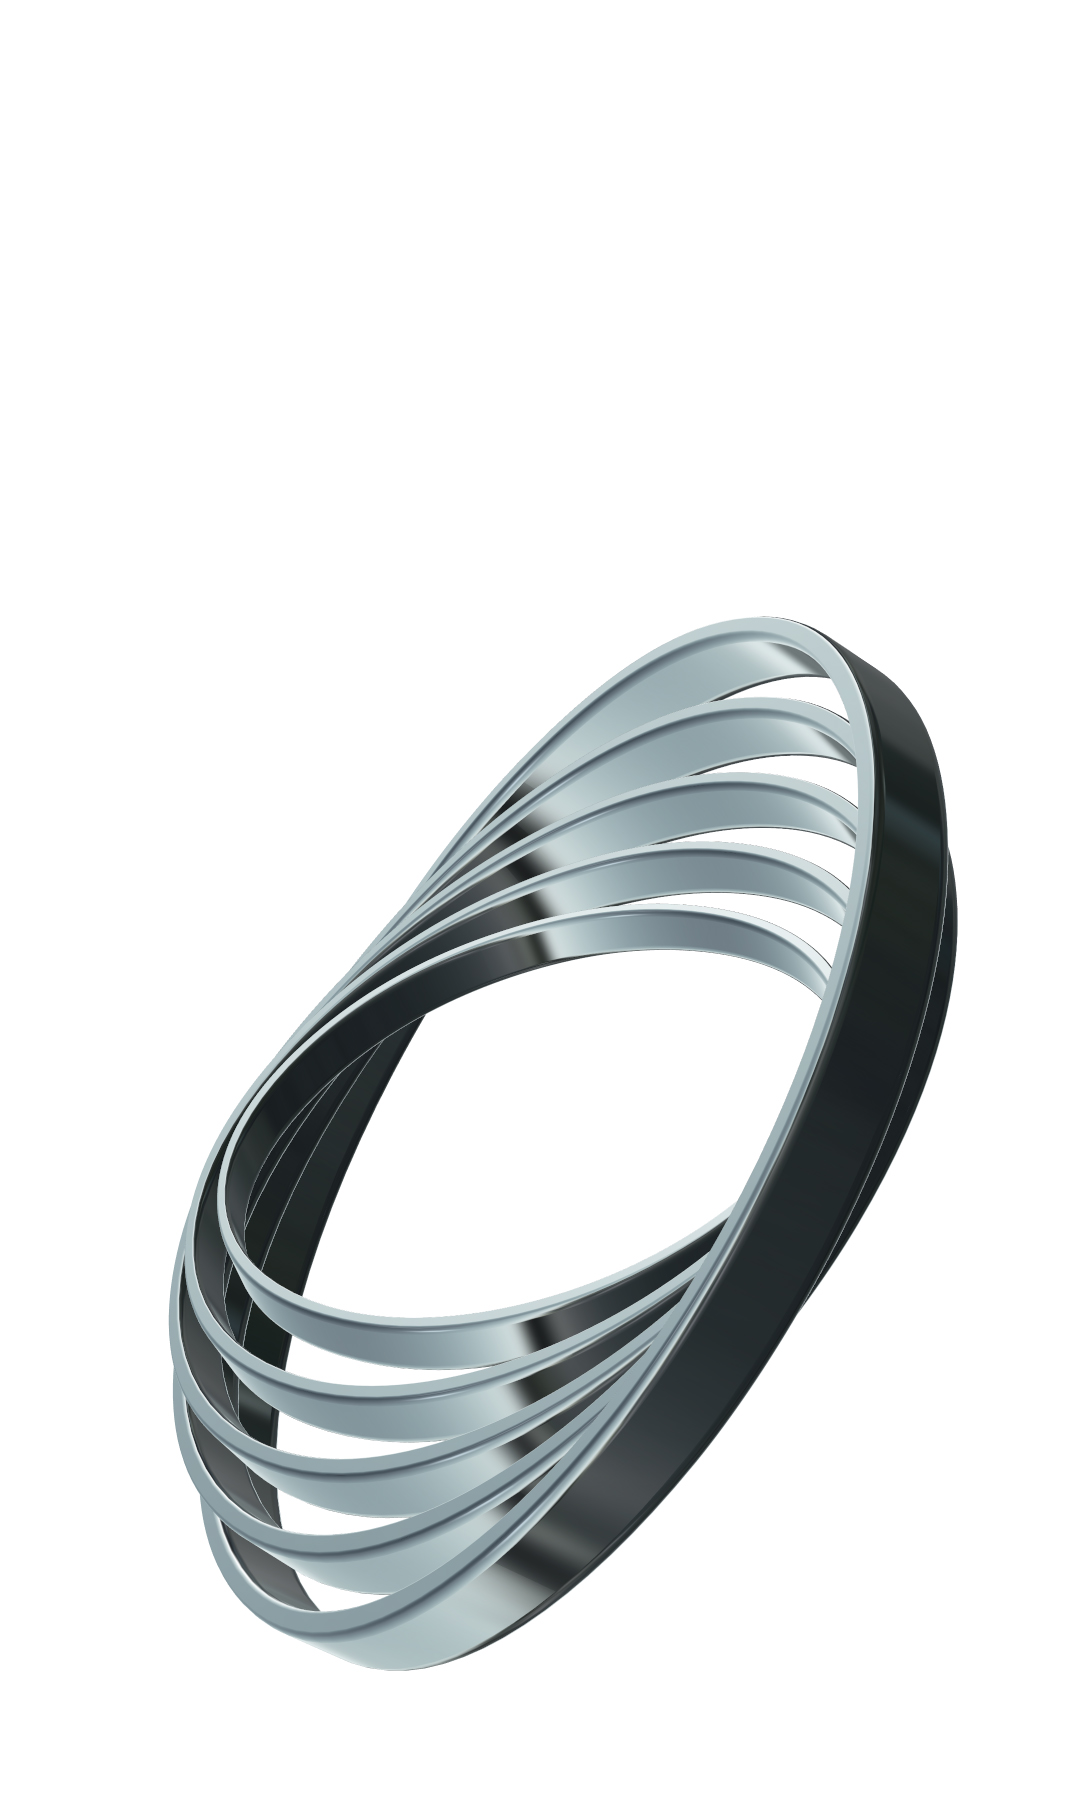
\includegraphics[trim={0 0 0 17cm},width=\paperwidth,height=\paperheight]{BG5.jpg}}
}
%----------------------------------------------------------------------------------------
%	NAME AND CONTACT INFORMATION SECTION
%----------------------------------------------------------------------------------------

\firstname{Human Being} % Your first name
\familyname{\#117,314,159,265} % Your last name

% All information in this block is optional, comment out any lines you don't need
\title{The World is a Playground}
\address{Spatial Coordinates (Tauien Standard)}{009.384:203.237:098.122:231.239:238.021}
\mobile{Intergalactic: ST:3}
%\phone{None}
\email{earthemail0027@gmail.com}
%\homepage{}{} % The first argument is the url for the clickable link, the second argument is the url displayed in the template - this allows special characters to be displayed such as the tilde in this example
%\extrainfo{Contact via e-mail is best}
%\photo[70pt][0.4pt]{pictures/picture_me} % The first bracket is the picture height, the second is the thickness of the frame around the picture (0pt for no frame)
%\quote{}

%----------------------------------------------------------------------------------------

\begin{document}

\makecvtitle % Print the CV title

%----------------------------------------------------------------------------------------
%	EDUCATION SECTION
%----------------------------------------------------------------------------------------

\section{Education}

\cventry{2010--Present}{College DLC.}{Earth}{Milkey Way Galaxy, Sol planet 3.}{\textit{GPA -- 1.2}}{Through Various Pottery and sports classes, I've managed to maximize my debt with minimal effort.}
\cventry{1992--2010}{Tutorial.}{Earth}{Milkey Way Galaxy, Sol planet 3.}{}{Through various challenges, I've managed to learn walking, talking, and other things through my superior knowledge and learning capabilities.}

%----------------------------------------------------------------------------------------
%	WORK EXPERIENCE SECTION
%----------------------------------------------------------------------------------------

\section{Experience}

%\subsection{Vocational}

\cventry{1992--Present}{Inhabitant of Earth}{Residence of Michigan}{United States}{}{Earth is hard. People are mean. I've had to toughen my skin and lock down my emotions to prevent against verbal offenses.}

%------------------------------------------------

\subsection{Miscellaneous}
\cventry{2002}{Grand Master Of the Peter Pan Clan}{Neighborhood Town}{}{}{After conquering the snow fortress of Billy, I was named Grand Master of our clan.}

%----------------------------------------------------------------------------------------
%	PUBLICATIONS \& PROJECTS
%----------------------------------------------------------------------------------------

\section{Projects}

\cvitem{2001}{Made some mud soup using materials scavenged from back yard.}
\cvitem{2001}{Created award winning blanket fortress.}
\cvitem{2000}{Broke a stick into three pieces and made a triangle (thus, self taught mathematician).}

%----------------------------------------------------------------------------------------
%	AWARDS SECTION
%----------------------------------------------------------------------------------------

\section{Clubs and Honors}

\cvitem{1999}{Became Spiritual Leader for a large colony of ants (at least 6 ants).}

%----------------------------------------------------------------------------------------
%	COMMUNICATION SKILLS SECTION
%----------------------------------------------------------------------------------------

%\section{Communication Skills}

%\cvitem{2011--2012}{Composition I/II classes with various presentations}
%\cvitem{2013}{REU Condensed Matter Research presentation}

%----------------------------------------------------------------------------------------
%	LANGUAGES SECTION
%----------------------------------------------------------------------------------------

%\section{Languages}

%\cvitemwithcomment{English}{Mothertongue}{}
%\cvitemwithcomment{German}{Basic}{Basic words and phrases only}
%\cvitemwithcomment{Japanese}{Basic}{Basic words and phrases only}

%----------------------------------------------------------------------------------------
%	INTERESTS SECTION
%----------------------------------------------------------------------------------------

\section{Interests and Hobbies}
\cvitem{}{Sleeping.}

%----------------------------------------------------------------------------------------
%	REFERENCES SECTION
%----------------------------------------------------------------------------------------

\section{References}

\cventry{1992--Present}{Human Being \#117,315,159,265}{}{}{}{Only human being capable of an accurate reference.}

%----------------------------------------------------------------------------------------
%	COVER LETTER
%----------------------------------------------------------------------------------------

% To remove the cover letter, comment out this entire block

%\clearpage

%\recipient{HR Department}{Corporation\\123 Pleasant Lane\\12345 City, State} % Letter recipient
%\date{\today} % Letter date
%\opening{Dear Sir or Madam,} % Opening greeting
%\closing{Sincerely yours,} % Closing phrase
%\enclosure[Attached]{curriculum vit\ae{}} % List of enclosed documents

%\makelettertitle % Print letter title

%\lipsum[1-3] % Dummy text

%\makeletterclosing % Print letter signature

%----------------------------------------------------------------------------------------

\end{document}